\documentclass[12pt,twoside]{article}
\usepackage[dvipsnames]{xcolor}
\usepackage{tikz,graphicx,amsmath,amsfonts,amscd,amssymb,bm,cite,epsfig,epsf,url}
\usepackage[hang,flushmargin]{footmisc}
\usepackage[colorlinks=true,urlcolor=blue,citecolor=blue]{hyperref}
\usepackage{amsthm,multirow,wasysym,appendix}
\usepackage{array,subcaption} 
% \usepackage[small,bf]{caption}
\usepackage{bbm}
\usepackage{pgfplots}
\usetikzlibrary{spy}
\usepgfplotslibrary{external}
\usepgfplotslibrary{fillbetween}
\usetikzlibrary{arrows,automata}
\usepackage{thmtools}
\usepackage{blkarray} 
\usepackage{textcomp}
\usepackage[left=0.8in,right=1.0in,top=1.0in,bottom=1.0in]{geometry}
\usepackage{pifont}
\newcommand{\tick}{\ding{51}}%
\newcommand{\xmark}{\ding{55}}
\input{macros}

\newcommand{\ru}{\rnd{ u}  }
\newcommand{\rd}{\rnd{ d}  }
%\newcommand{\rs}{\rnd{ s}  }
\newcommand{\ri}{\rnd{ i}  }
\newcommand{\re}{\rnd{ e}  }
\newcommand{\rQ}{\rnd{ q}  }
\newcommand{\rC}{\rnd{ c}  }
\newcommand{\red}[1]{{\leavevmode\color{red}{#1}}}
\newcommand{\blue}[1]{{\leavevmode\color{blue}{#1}}}
\usepackage{graphicx}

\begin{document}

\begin{center}
{\large{\textbf{Homework 6}} } \vspace{0.2cm}\\
Due October 30 at 11 pm
\\
\end{center}
\input{hwstatement.tex}\\

\begin{enumerate}

\item (Spam detector) In order to build a spam classifier, we gather the following data. Each row is an email. The first column indicates whether it is spam or not. The remaining columns indicate whether it contains (\tick) or not (\xmark) the word on top.
\begin{center}
{\footnotesize
\begin{tabular}{ |c|c|c|c|c| } 
 \hline
 & Miracle  & Alternative & Medicine & Basketball \\
\hline 
Spam &  \tick  & \tick& \tick & \tick  \\
\hline
Not spam &  \xmark  & \xmark& \tick & \tick  \\
\hline 
Spam &  \tick  & \xmark& \xmark & \xmark  \\
\hline
Not spam &  \xmark  & \tick& \xmark & \xmark  \\
\hline
Spam &  \tick  & \xmark& \xmark & \xmark  \\
\hline
Not spam &  \xmark  & \tick& \xmark & \tick  \\
\hline 
Spam &  \tick  & \xmark& \xmark & \xmark  \\
\hline
Spam &  \xmark  & \tick& \tick & \xmark  \\
\hline
Not spam &  \tick  & \tick& \xmark & \tick  \\
\hline
Not spam &  \xmark  & \xmark& \tick & \tick  \\
\hline 
\end{tabular}
}
\end{center}
We use a Bernoulli random variable $\ry$ to model whether the email is spam ($\ry=1$) or not ($\ry=0$), and a four-dimensional random vector $\rx$ to indicate whether the $i$th word is  ($\rx[i]=1$) or not ($\rx[i]=0$) in the email for $i \in \keys{1,2,3,4}$.
\begin{enumerate}
\item  Your friend recommends that you estimate the conditional pmf of $\ry$ given $\rx$ and then maximize it to produce your estimate. What is the problem with this approach?

\red{\begin{itemize}
    \item we have 8 total observations. 
    \item without making any assumptions there are 4 features and 2 classes, so we there are $2^4=16$ parameters to estimate and we only have 10 data points. 
    \item so this estimation would be infeasible
\end{itemize}}
\item Apply naive Bayes to classify an email that reads \emph{I hurt my foot playing basketball. %It's a miracle I didn't break it. 
Can you get me some medicine?} 
\red{
\begin{itemize}
    \item the sentence, "I hurt my foot playing basketball." can be encoded as $x=\{\tilde{x_1}=0,\tilde{x_2}=0,\tilde{x_3}=1,\tilde{x_4}=1\}$
    \item under naive bays we assume that $x_1...x_4$ are conditionally independent given y, thus we can write $P(\tilde{y}=1|\tilde{x_1}=0,\tilde{x_2}=0,\tilde{x_3}=1,\tilde{x_4}=1)=\\\frac{P(\tilde{y}=1,\tilde{x_1}=0,\tilde{x_2}=0,\tilde{x_3}=1,\tilde{x_4}=1)}{P(\tilde{y}=1,\tilde{x_1}=0,\tilde{x_2}=0,\tilde{x_3}=1,\tilde{x_4}=1)+P(\tilde{y}=0,\tilde{x_1}=0,\tilde{x_2}=0,\tilde{x_3}=1,\tilde{x_4}=1)}=\frac{P(\tilde{y}=1)\Pi_{i=1}^{4}P(\tilde{x}[i]=x_i|\tilde{y}=1)}{\Sigma_{w=0}^{1}P(\tilde{y}=w)\Pi_{i=1}^{4}P(\tilde{x}[i]=x_i|\tilde{y}=w)}=\frac{3}{35}$
    \item this tells us that $P(\tilde{y}=0|\tilde{x}=x)>P(\tilde{y}=1|\tilde{x}=x)$ thus we would classify the email as ham 
\end{itemize}
}
\item Apply naive Bayes to classify an email that reads \emph{This alternative medicine is amazing, send us all your money!} Explain what shortcoming of the naive Bayes classifier is illustrated by this example.
\end{enumerate}
\begin{itemize}
     
\item we can think of x in this case as $X=\{x_1=0,x_2=1,x_3=1,x_4=0\}$
\item so we can see that $P(\tilde{y}=1|\tilde{x}=x)=\frac{P(\tilde{y}=1)\Pi_{i=1}^{4}P(\tilde{x}[i]=x[i]|y=1)}{\Sigma_{1=0}^{1}P(\tilde{y}=w)\Pi_{i=1}^{4}P(\tilde{x}[i]=x[i]|y=w)}=\frac{\frac{1}{2}(\frac{1}{5}\frac{2}{5}\frac{2}{5}\frac{4}{5})}{\frac{1}{2}(\frac{1}{5}\frac{2}{5}\frac{2}{5}\frac{4}{5}+\frac{4}{5}\frac{3}{5}\frac{2}{5}\frac{1}{5})}=\frac{2}{5}$
 \item this tells us that $P(\tilde{y}=0|\tilde{x}=x)>P(\tilde{y}=1|\tilde{x}=x)$ thus we would not classify the email as spam 
 \item this illustrates the issue that naive Bayes only works when there is actually conditional Independence between the features. In this case this clearly does not hold as emails containing alternative medicine (are likely to be scams) 
\end{itemize}

\item (The Markov property) Let $\ra_1$, $\ra_2$, \ldots, $\ra_n$ be a Markov chain, where for any $1 < i < n$, $\ra_{i+1}$ is conditionally independent of $\ra_1 ,\ldots,\ra_{i-1}$ given $\ra_{i}$, i.e.
\begin{align}
\label{eq:markov_cond_pmf}
p_{ \ra_{ i+1} \cnd \ra_1 ,\ldots,\ra_{i}  }\brac{ a_{i+1} \cnd a_1, a_2, \ldots, a_i } =  p_{ \ra_{i+1}  \cnd \ra_i  }\brac{ a_{ i+1} \cnd a_{i} },
\end{align}
for any values of $a_1$, $a_2$, \ldots, $a_n$. Show that this implies that the future is conditionally independent from the past given the present:
\begin{align}
p_{ \ra_{ i+1},\ra_{i-1} \cnd \ra_i }\brac{ a_{i+1},a_{i-1} \cnd  a_i } = p_{ \ra_{ i+1} \cnd \ra_i }\brac{ a_{i+1} \cnd  a_i } p_{ \ra_{i-1} \cnd \ra_i }\brac{ a_{i-1} \cnd  a_i },
\end{align}
for any $2 \leq i \leq n-1$ and any values of $a_{i-1}$, $a_i$, $a_{i+1}$. (Hint: First show that $p_{ \ra_{ i+1} \cnd \ra_{i-1} , \ra_i}\brac{ a_{i+1}\cnd a_{i-1}, a_{i}  }  = p_{ \ra_{ i+1} \cnd  \ra_i}\brac{ a_{i+1}\cnd a_{i}  } $ for $a_{i-1}$, $a_i$, $a_{i+1}$.)

\red{
\begin{itemize}
    \item notice first as we know $\Tilde{a}_{i+1}, \Tilde{a}_{i-1}$ are conditionally independent given $\Tilde{a}_i$ we know that $P_{\Tilde{a}_{i+1}|\Tilde{a}_{i-1},\Tilde{a}_{i}}(a_{i+1}|a_{i},a_{i-1})=P_{\Tilde{a}_{i+1}|\Tilde{a}_{i}}(a_{i+1}|a_{i})$ that is just be definition 
    \item now observe that we can express $P_{\Tilde{a}_{i+1},\Tilde{a}_{i-1}|\Tilde{a}_{i}}(a_{i+1},a_{i-1}|a_{i})=\frac{P_{\Tilde{a}_{i+1},\Tilde{a}_{i-1},\Tilde{a}_{i}}(a_{i+1},a_{i-1},a_{i})}{P_{\Tilde{a}_{i}}(a_{i})}=\frac{P_{\Tilde{a}_{i+1}|\Tilde{a}_{i-1},\Tilde{a}_{i}}(a_{i+1}|a_{i-1},a_{i})*P_{\Tilde{a}_{i-1},\Tilde{a}_{i}}(a_{i-1},a_{i})}{P_{\Tilde{a}_{i}}(a_{i})}=\frac{P_{\Tilde{a}_{i+1}|\Tilde{a}_{i-1},\Tilde{a}_{i}}(a_{i+1}|a_{i-1},a_{i})*P_{\Tilde{a}_{i-1}|\Tilde{a}_{i}}(a_{i-1}|a_{i})*P_{\Tilde{a}_{i}}(a_{i})}{P_{\Tilde{a}_{i}}(a_{i})}\\=P_{\Tilde{a}_{i+1}|\Tilde{a}_{i-1},\Tilde{a}_{i}}(a_{i+1}|a_{i-1},a_{i})*P_{\Tilde{a}_{i-1}|\Tilde{a}_{i}}(a_{i-1}|a_{i})$ and as we showed above 
    $P_{\Tilde{a}_{i+1}|\Tilde{a}_{i-1},\Tilde{a}_{i}}(a_{i+1}|a_{i},a_{i-1})=P_{\Tilde{a}_{i+1}|\Tilde{a}_{i}}(a_{i+1}|a_{i})$
    \item meaning that $P_{\Tilde{a}_{i+1},\Tilde{a}_{i-1}|\Tilde{a}_{i}}(a_{i+1},a_{i-1}|a_{i})=P_{\Tilde{a}_{i+1}|\Tilde{a}_{i}}(a_{i+1}|a_{i})P_{\Tilde{a}_{i-1}|\Tilde{a}_{i}}(a_{i-1}|a_{i})$
     \square
\end{itemize}
}

\item (Mobile phones)
A company that makes mobile phones wants to model the sales of a new model they have just released. At the moment 90\% of the phones are in stock, 10\% have been sold locally and none have been exported. Based on past data, the company determines that each day a phone is sold with probability 0.2 and exported with probability 0.1. We define the following time-homogeneous Markov chain with three states to model this:

\begin{center}
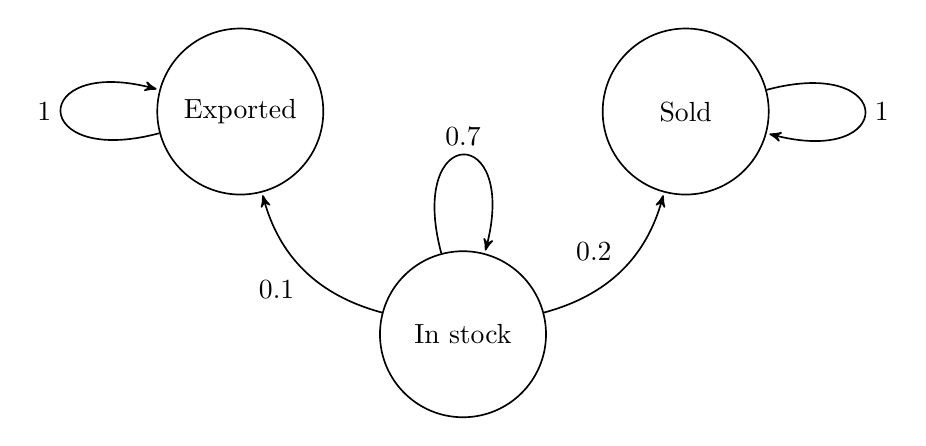
\begin{tikzpicture}[->,>=stealth',shorten >=1pt,auto,node distance=4cm,
                    semithick]
  \tikzstyle{every state}=[text=black]

 \node[state,minimum size = 60pt] (S)                    {In stock};
  \node[state,minimum size = 60pt]         (C) [above right of=S] {Sold};
  \node[state,minimum size = 60pt]         (G) [above left of=S] {Exported};
 
  \path (S) edge    [bend right]      node {0.2} (C)
            edge     [bend left]         node {0.1} (G)
            edge [loop above] node {0.7} (S)
        (C) edge [loop right] node  {1} (C)
        (G) edge [loop left] node  {1} (G);
\end{tikzpicture}
\end{center} 

\begin{enumerate}
\item What is the limit of the state vector $\pi_{i}$ as $i \rightarrow \infty$?
\red{
\begin{itemize}
    \item we can write our transition matrix $T\in \mathbb{R}^{3}$ as $T=$\begin{pmatrix}1,&.1,&0\\0,&.7&,0\\0,&.2,&1
    \end{pmatrix}
    \item we can also write our given intitial state as $\pi_0=\begin{pmatrix} 0\\.9 \\.1 \end{pmatrix}$
    \item then notice that long term behavior as $lim_{t\rightarrow \infty}\pi_i=lim_{t\rightarrow \infty}T^{i}\pi_0=lim_{t\rightarrow \infty}Q\Lambda^{i}Q^{-1}\pi_0=lim_{t\rightarrow \infty}Q\begin{pmatrix}1&0&0\\0&1&0\\0&0&.7\end{pmatrix}^{i}Q^{-1}\pi_0=Q\begin{pmatrix}1&0&0\\0&1&0\\0&0&0\end{pmatrix}Q^{-1}\pi_0=\begin{pmatrix}.3\\0\\.7\end{pmatrix}$
    \item where Q is an orthogonal matrix with eigenvectors of T and lambda is a diagonal matrix with the corresponding eigenvalues of T. I chose not to write out Q in this page, just because it makes the page a lot messier with out really increasing clarity. 
    \item this makes sense intuitively as we know that we start with 90 precetn of the phones in stock and 10 percent sold. then in teh long term we would expcet that 2/3 of what is in stock (ie) and additional 60 percent would be sold and 1/3 of what is in stock ie 30 percent to be exported  
\end{itemize}
}

\item Simulate the Markov chain and plot the evolution of the state vector. 
\red{
\item as we can see here simulating the behavior results in the expected long term state 
\\\includegraphics[width=15cm]{homework 6/homework 6 immage 1.png}
}
\end{enumerate}

\item (Smoothing) In the application of naive Bayes, instead of computing the conditional pmf $p_{\rnd{x}[i] \cnd \rnd{y}}(x[i]|y)$ empirically, we usually compute the conditional pmf as follows:

$$p_{\rnd{x}[i] \cnd \rnd{y}}(\rnd{x}[i] \cnd y) = \frac{\text{number of samples with label } y \text{ and having feature } x[i] + m}{\text{number of samples with label } y + md},$$

where $m$ is a smoothing constant, and $d$ is the number of features.

\begin{enumerate}
 \item What is the problem with naive Bayes when there is no smoothing ($m=0$) and how does smoothing alleviate this?
 \begin{itemize}
     
 \item using empirical probability and naive bays we estimate the joint probably as the product of marginal probabilities. so if something never appears in our data, we estimate its marginal probability as zero, meaning that its joint probability with anything else will be zero. this type of smoothing, shifts that number to a slightly positive value, so that it is small but not zero and thus does not cause our entire product to be zero . 
  \end{itemize}

  \item Complete the notebook \textit{spam.ipynb}. Which $m$ results in the highest accuracy on the test set?

      
  \red{
    \begin{itemize}
        \item i got my max at m=0, i have attached my code to this file. this solution sounds kind of wrong to me though 
       \end{itemize}
      }
  \item In the code, we compare the joint pmf $p_{\rnd{y}, \rnd{x}[1], \cdots, \rnd{x}[d]}(y, \rnd{x}[1], \cdots \rnd{x}[d])$ for $y\in \{0,1\}$. Why is this equivalent to Equation (4.146) in the notes? Why do we need to apply the logarithm in practice?
  \begin{itemize}
    
    \item this equality holds because we are making iid assumptions $P(\tilde{y}=y,\tilde{x_1}=x,..,\tilde{x_n}=x)=P(\tilde{x_n}=x|\tilde{y}=y,,..,\tilde{x_{n-1}}=x)P(\tilde{y}=y,,..,\tilde{x_{n-1}}=x)=P(\tilde{x_n}=x|\tilde{y}=y)P(\tilde{x_{n-1}}=x|\tilde{y}=y, \tilde{x_1}=x,...\tilde{x_{n-2}}=x)=...=P(x_n=x|y)P(x_{n-1}=x|y)...P(x_1|y)p(y)$ and furhter since the denominator is the same for y= and y=1
      \item firstly due to Laplace smoothing we should never get values that are equal to zero, so the probability is strictly positive in this case and thus the log is well defined on the domain 
      \item secondly we are only interested in the max of the function on this interval, and log is increasing so this transformation will not effect our max
      \item third we are dealing with the products of many values between 0 and 1 so takign the log allows us to take the sum of these vallues meaning our computer deos not have to deal with floating point issues.
    
  \end{itemize}
  \\\includegraphics[width=15cm]{homework 6/homework 6 immage 2.png.jpg}
  \\\includegraphics[width=15cm]{homework 6/homework 6 immage 3.png.jpg}
  \\\includegraphics[width=15cm]{homework 6/homework 6 immage 4.png.jpg}
  
 
\end{enumerate}


\end{enumerate}
\end{document}
